%%%%%%%%%%%%%%%%%%%%%%%%%%%%%%%%%%%
%This is the LaTeX COMMUNICATION template for RSC journals
%Copyright The Royal Society of Chemistry 2016
%%%%%%%%%%%%%%%%%%%%%%%%%%%%%%%%%%%

\documentclass[twoside,twocolumn,9pt]{article}
\usepackage{extsizes}
\usepackage[super,sort&compress,comma]{natbib} 
\usepackage[version=3]{mhchem}
\usepackage[left=1.5cm, right=1.5cm, top=1.785cm, bottom=2.0cm]{geometry}
\usepackage{balance}
\usepackage{mathptmx}
\usepackage{sectsty}
\usepackage{graphicx} 
\usepackage{lastpage}
\usepackage[format=plain,justification=justified,singlelinecheck=false,font={stretch=1.125,small,sf},labelfont=bf,labelsep=space]{caption}
\usepackage{float}
\usepackage{fancyhdr}
\usepackage{fnpos}
\usepackage[english]{babel}
\addto{\captionsenglish}{%
  \renewcommand{\refname}{Notes and references}
}
\usepackage{array}
\usepackage{droidsans}
\usepackage{charter}
\usepackage[T1]{fontenc}
\usepackage[usenames,dvipsnames]{xcolor}
\usepackage{setspace}
\usepackage[compact]{titlesec}
\usepackage{hyperref}
%%%Please don't disable any packages in the preamble, as this may cause the template to display incorrectly.%%%


\usepackage{epstopdf}%This line makes .eps figures into .pdf - please comment out if not required.

\definecolor{cream}{RGB}{222,217,201}
%%%%%%%%% Preamble of the bibliography, can be commented or deleted 
\def\bibpreamble{For the reference section, the style file \texttt{rsc.bst} can be used to generate the correct reference style.\footnote[4]{Footnotes should appear here. These might include comments relevant to but not central to the matter under discussion, limited experimental and spectral data, and crystallographic data.}
\begin{enumerate}
\item{Citations should appear here in the format A. Name, B. Name and C. Name, \emph{Journal Title}, 2000, \textbf{35}, 3523;} 
\item{A. Name, B. Name and C. Name, \emph{Journal Title, 2000}, \textbf{35}, 3523.}
\end{enumerate}
... \\\\
We encourage the citation of primary research over review articles, where appropriate, in order to give credit to those who first reported a finding. \href{https://www.rsc.org/news-events/articles/2020/jun/rsc-signs-dora/}{Find out more about our commitments to the principles of San Francisco Declaration on Research Assessment (DORA).}}
%%%%%%%%% 
\begin{document}

\pagestyle{fancy}
\thispagestyle{plain}
\fancypagestyle{plain}{
%%%HEADER%%%
\renewcommand{\headrulewidth}{0pt}
}
%%%END OF HEADER%%%

%%%PAGE SETUP - Please do not change any commands within this section%%%
\makeFNbottom
\makeatletter
\renewcommand\LARGE{\@setfontsize\LARGE{15pt}{17}}
\renewcommand\Large{\@setfontsize\Large{12pt}{14}}
\renewcommand\large{\@setfontsize\large{10pt}{12}}
\renewcommand\footnotesize{\@setfontsize\footnotesize{7pt}{10}}
\renewcommand\scriptsize{\@setfontsize\scriptsize{7pt}{7}}
\makeatother

\renewcommand{\thefootnote}{\fnsymbol{footnote}}
\renewcommand\footnoterule{\vspace*{1pt}% 
\color{cream}\hrule width 3.5in height 0.4pt \color{black} \vspace*{5pt}} 
\setcounter{secnumdepth}{5}

\makeatletter 
\renewcommand\@biblabel[1]{#1}            
\renewcommand\@makefntext[1]% 
{\noindent\makebox[0pt][r]{\@thefnmark\,}#1}
\makeatother 
\renewcommand{\figurename}{\small{Fig.}~}
\sectionfont{\sffamily\Large}
\subsectionfont{\normalsize}
\subsubsectionfont{\bf}
\setstretch{1.125} %In particular, please do not alter this line.
\setlength{\skip\footins}{0.8cm}
\setlength{\footnotesep}{0.25cm}
\setlength{\jot}{10pt}
\titlespacing*{\section}{0pt}{4pt}{4pt}
\titlespacing*{\subsection}{0pt}{15pt}{1pt}
%%%END OF PAGE SETUP%%%

%%%FOOTER%%%
\fancyfoot{}
\fancyfoot[LO,RE]{\vspace{-7.1pt}
\includegraphics[height=9pt]{head_foot/LF}}
\fancyfoot[CO]{\vspace{-7.1pt}\hspace{13.2cm}
\includegraphics{head_foot/RF}}
\fancyfoot[CE]{\vspace{-7.2pt}\hspace{-14.2cm}
\includegraphics{head_foot/RF}}
\fancyfoot[RO]{\footnotesize{\sffamily{1--\pageref{LastPage} ~\textbar  \hspace{2pt}\thepage}}}
\fancyfoot[LE]{\footnotesize{\sffamily{\thepage~\textbar\hspace{3.45cm} 1--\pageref{LastPage}}}}
\fancyhead{}
\renewcommand{\headrulewidth}{0pt} 
\renewcommand{\footrulewidth}{0pt}
\setlength{\arrayrulewidth}{1pt}
\setlength{\columnsep}{6.5mm}
\setlength\bibsep{1pt}
%%%END OF FOOTER%%%

%%%FIGURE SETUP - please do not change any commands within this section%%%
\makeatletter 
\newlength{\figrulesep} 
\setlength{\figrulesep}{0.5\textfloatsep} 

\newcommand{\topfigrule}{\vspace*{-1pt}% 
\noindent{\color{cream}\rule[-\figrulesep]{\columnwidth}{1.5pt}} }

\newcommand{\botfigrule}{\vspace*{-2pt}% 
\noindent{\color{cream}\rule[\figrulesep]{\columnwidth}{1.5pt}} }

\newcommand{\dblfigrule}{\vspace*{-1pt}% 
\noindent{\color{cream}\rule[-\figrulesep]{\textwidth}{1.5pt}} }

\makeatother
%%%END OF FIGURE SETUP%%%

%%%TITLE AND AUTHORS%%%
\twocolumn[
  \begin{@twocolumnfalse}
{
\includegraphics[height=30pt]{head_foot/journal_name}\hfill\raisebox{0pt}[0pt][0pt]{
\includegraphics[height=55pt]{head_foot/RSC_LOGO_CMYK}}\\[1ex]

\includegraphics[width=18.5cm]{head_foot/header_bar}}\par
\vspace{1em}
\sffamily
\begin{tabular}{m{4.5cm} p{13.5cm} }


\includegraphics{head_foot/DOI} & \noindent\LARGE{\textbf{A Green, Solvent-Saving Analytical Strategy for Equivalence Point Determination in Potentiometric Titrations via Gran and Schwartz Linearization$^\dag$}} \\%Article title goes here instead of the text "This is the title"
 & \vspace{0.3cm} \\

 & \noindent\large{Samuele Giani,$^{\ast}$\textit{$^{a}$} and Cosimo A. De Caro,$^{\ast}$\textit{$^{b}$}} \\%Author names go here instead of "Full name", etc.

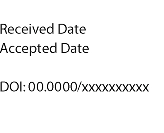
\includegraphics{head_foot/dates} & \\

\end{tabular}

 \end{@twocolumnfalse} \vspace{0.6cm}

  ]
%%%END OF TITLE AND AUTHORS%%%

%%%FONT SETUP - please do not change any commands within this section
\renewcommand*\rmdefault{bch}\normalfont\upshape
\rmfamily
\section*{}
\vspace{-1cm}


%%%FOOTNOTES%%%

\footnotetext{\textit{$^{a}$~Universitätsspital Zürich, Rämistrasse 100, 8091 Zürich, Switzerland. E-mail: samuele.giani@usz.ch}}
\footnotetext{\textit{$^{b}$~Mettler--Toledo GmbH Analytical, Heuwinkelstrasse 3, 8606 Nänikon, Switzerland. E-mail: cosimo.decaro@mt.com}}

%Please use \dag to cite the ESI in the main text of the article.
%If you article does not have ESI please remove the the \dag symbol from the title and the footnotetext below.
\footnotetext{\dag~Supplementary Information available: [details of any supplementary information available should be included here]. See DOI: 00.0000/00000000.}
%additional addresses can be cited as above using the lower-case letters, c, d, e... If all authors are from the same address, no letter is required

%\footnotetext{\dag~Additional footnotes to the title and authors can be included \textit{e.g.}\ `Present address:' or `These authors contributed equally to this work' as above using the symbols: \ddag, \textsection, and \P. Please place the appropriate symbol next to the author's name and include a \texttt{\textbackslash footnotetext} entry in the the correct place in the list.}

%%%END OF FOOTNOTES%%%

%%%ABSTRACT%%%%

\sffamily{\textbf{Potentiometric titrations remain a cornerstone of analytical chemistry however require excessive titrant and solvent volumes due to the need for full-curve exploration to locate the equivalence point (EQP), contributing to unnecessary waste and contradicting green chemistry principles. Here, we introduce a sustainable two-step analytical strategy that systematically reduces solvent consumption while maintaining high accuracy in EQP determination.
An initial conventional titration with titrant addition identifies the pre-equivalence linear region via Gran and Schwartz linearization methods. The central point of this linear segment serves as the truncation limit for subsequent measurements. Follow-up titrations employ smaller fixed increments only up to this limit, enabling precise EQP extrapolation from the limited linear data.
Applied to the aqueous titration of TRIS with \ce{HCl}, this approach yields EQP values with excellent repeatability (standard error comparable to or better than traditional full-titration methods across n=6 replicates each). Solvent consumption is reduced by 15-20\% per analysis (e.g., approximately 1 mL saved relative to reaching the EQP of 5 mL), directly supporting Principles 1, 5, and 8 of green chemistry.
Implemented in the open-source Python tool GranTED (available at https://github.com/sgiani95/GranTED), this protocol offers a practical, low-waste alternative for routine and educational potentiometric analyses.}\\%The abstrast goes here instead of the text "The abstract should be..."

%%%END OF ABSTRACT%%%%

\rmfamily %Please do not remove this line.

%%%MAIN TEXT%%%%

\section*{Introduction}

Potentiometric titrations are a cornerstone of analytical chemistry for determining equivalence points (EQPs). All methods rely on identifying the inflection point in E or pH versus volume of added titrant ($V$) curves, but these often suffer from low accuracy in systems with small potential steps, such as weak electrolytes or asymmetric curves. To address this, Gran introduced differential plotting of $\Delta V/\Delta E$ or $\Delta V/\Delta pH$ versus $V$ in 1950, yielding near-linear segments intersecting at the EQP. In 1952, Gran refined this with antilogarithmic transformations (e.g., $V × 10^{-pH}$ versus $V$), producing straight lines for easier extrapolation. Schwartz further advanced Gran methodology in 1987 by incorporating corrections for significant \ce{[H+]}/\ce{[OH-]} effects enabling analysis of challenging cases.

Despite these methodological improvements, potentiometric titrations remain resource-intensive, always requiring full-curve acquisitions that consume excess solvent, generating unnecessary waste contrary to green chemistry principles (i.e., waste prevention). Herein, we present a sustainable analytical strategy that minimizes solvent use while leveraging Gran (1952) and Schwartz linearizations for precise EQP determination.

The analytical protocol involves an initial conventional titration with titrant addition to identify the pre-EQP linear region. The central point of this segment then defines the truncation limit for subsequent titrations using smaller fixed increments, enabling EQP extrapolation from decreased-volume data. Applied to TRIS-\ce{HCl} titrations (n=6 replicates per condition), this yields EQPs with repeatability comparable to traditional full titrations but with 15–20\% solvent reduction per analysis (e.g., approximately 1 mL saved versus 5 mL EQP or even more considering full endpoint). This approach supports Principles of Green Chemistry 1, 5, and 8, offering a greener tool for routine and educational analyses. Open-source implementation in Python (GranTED, GitHub) facilitates adoption.

\section*{Experimental Section}

\subsection*{Materials and Instrumentation}

Tris(hydroxymethyl)aminomethane (TRIS, 99.97\%, Merck Sigma-Aldrich) was titrated with hydrochloric acid (\ce{HCl}, 0.1 M).
%, standardized against Na₂CO₃). Solutions were prepared in deionized water (18.2 MΩ·cm) with 0.1 M KCl as supporting electrolyte to maintain constant ionic strength (μ ≈ 0.1 M). 
Potentiometric measurements used a Mettler Toledo autoburette with a glass electrode. % (Ag/AgCl reference, calibrated with HCl/NaOH standards in the same medium to read -log[H⁺]). Titrant addition employed a Mettler Toledo T5 burette (precision ±0.005 mL).
All experiments were conducted at room temperature. %25 ± 0.5 °C under N₂ atmosphere to minimize CO₂ interference.

\subsection*{Protocols}

Initial dynamic titration: 5 mL TRIS (0.1 M), diluted with 60 mL deionized water, with variable \ce{HCl} increments (0.5–1 mL pre-buffer, 0.05 mL near EQP) until post-EQP. Data processed via Schwartz-modified Gran plots to identify pre-EQP linear region ($R^2$ > 0.999) and central point. Validation: n=6 replicates with fixed 0.05 mL increments up to truncation. EQP extrapolated from linear fits; uncertainties from regression.

\subsection*{Data Analysis}

Implemented in Python-based GranTED (v1.0, MIT license, https://github.com/sgiani95/GranTED). Statistics: mean ± SD (n=6); savings calculated as volume differences vs. EQP/endpoint. Full equations, raw data, and pseudocode in Electronic Supporting Information (ESI).

\section*{Results and Discussion}

\subsection*{Method Development: Dynamic Titration for Linear Range Identification}

The sustainable analytical strategy begins with a single conventional dynamic titration to establish the baseline $pH-V$ curve and identify the pre-equivalence linear region necessary for subsequent truncations. For the titration of 5 mL of TRIS (0.1 M), diluted with 60 mL deionized water, with \ce{HCl} (0.1 M), the initial dynamic run (Figure 1a) yields a sigmoidal curve typical of weak base-strong acid systems ($pK_a$(TRIS) $\approx$ 8.1). Applying the Schwartz-modified Gran transformation ($(V+k) × 10^{-pH}$ vs. $V$, Figure 1b) linearizes the pre-EQP segment.%, as derived from Gran's 1952 antilog approach³ but adjusted for ion concentration effects to minimize curvature in moderately weak systems.
The linear region (shaded in Figure 1b) spans approximately [P–Q] mL, with its central point ([R] mL) determined via automated fitting ($R^2$ > 0.9995). This point, safely before the EQP to avoid overshoot, serves as the truncation limit for validations, reducing titrant waste while enabling extrapolation-based EQP determination akin to Gran's functions intersections.

\subsection*{EQP Determination via Extrapolation}

Extrapolation from the pre-EQP linear fit provides the EQP without requiring full post-equivalence data. In the dynamic run, the Schwartz plot (Figure 1b) intersects the V-axis at 5 mL (theoretical EQP), with uncertainty propagated from linear regression (± [0.1] mL). This aligns with Gran's 1952 theory for transforming parabolic branches into straight lines, enhanced by Schwartz's electroneutrality adjustments to account for \ce[H+] dominance in the buffer region. For TRIS-\ce{HCl}, the method yields precise EQPs even in noisy data, as the linear slope reflects system strength (steeper for stronger interactions). The central truncation point ensures the fit uses only reliable pre-EQP data.

\subsection*{Method Validation: High-Resolution Fixed-Increment Titration}

Subsequent validations confirm the strategy's accuracy using fixed smaller increments (e.g., 0.05 mL) up to the truncation point (Figure 1c). The corresponding Schwartz plot (Figure 1d) mirrors the dynamic linearization, extrapolating to an EQP of 5 mL (± 0.005 mL), matching the full-run value within experimental error. Across n=6 replicates per method, repeatability is excellent: standard deviation for truncated EQPs (0.0XX mL) is comparable to conventional full titrations ([0.0XX] mL; Table 1). Standard errors remain low (0.005\%), demonstrating robustness against volume variability. This validation echoes Schwartz's simulations for weak acids, where modified plots straighten curvature, but extends it to a practical truncation protocol for real-world efficiency.

\subsection*{Green Chemistry Metrics and Sustainability Assessment}

The truncation yields systematic solvent/titrant savings, quantified as 1 mL vs. the EQP and 1.5 mL vs. the full illustrative endpoint per analysis (Figure 2; [A\%] and [B\%] reductions, respectively). For routine labs performing multiple replicates, this accumulates to significant waste minimization, directly embodying Green Chemistry Principle 1 (prevention) by avoiding unnecessary full runs, Principle 5 (safer/less solvents) through reduced \ce{HCl} exposure, and Principle 8 (reduced derivatives) by minimizing buffer waste. Compared to traditional methods requiring exhaustive curves, our approach decreases resource use without compromising precision (Table 1). Implemented in the open-source Python tool GranTED, this facilitates automated linear detection and metrics calculation, promoting adoption in educational and monitoring contexts where sustainability is paramount.

%%%%%%%%%%%%%%%%%%%%%%%%

In the method development step, an initial dynamic titration (Figure 1a) reveals the raw sigmoidal pH curve, from which the pre-EQP linear region is identified via the Schwartz-modified Gran transformation (Figure 1b; eq. 1 from ref. 4). The central point of this linear segment (approximately at 4 mL) defines the truncation limit, enabling subsequent validations with fixed increments (Figure 1c) and same linear extrapolation (Figure 1d), achieving comparable EQP values (5 mL) with now minimized solvent use.

\begin{figure*}
\centering
  \includegraphics[height=3cm]{example2}
  \caption{Overview of the green analytical strategy for equivalence point (EQP) determination in potentiometric titrations, demonstrated for TRIS (0.1 M) titrated with \ce{HCl} (0.1 M). Left: (a) Raw pH vs. titrant volume (V) curve from the initial dynamic titration (full run to post-EQP), identifying the pre-EQP linear region (shaded) and its central truncation point (arrow). (b) Schwartz-modified Gran plot ($V × 10^{-pH}$ vs. $V$), showing the straight pre-EQP line extrapolated to the EQP (dashed line; intercept at 5 mL). Right: (c) Truncated validation titration: pH vs. V with fixed smaller increments up to the truncation point. (d) Corresponding Schwartz-modified plot for the truncated data, confirming EQP extrapolation (intercept at 5 mL) with reduced volume range.}
  \label{fig:titrations}
\end{figure*}

The truncated approach maintains analytical performance while substantially reducing resource consumption, as evidenced by the volume comparisons (Figure 2; mean savings of 1 mL vs. EQP and 1.5 mL vs. endpoint across replicates), directly supporting green chemistry Principles 1 and 5 through waste prevention and solvent minimization.

\begin{figure}[h]
\centering
  \includegraphics[height=3cm]{example1}
  \caption{Comparison of solvent/titrant volumes used in full vs. truncated validation titrations for TRIS-\ce{HCl} aqueous system (n=6 replicates each; mean ± SE). Savings are marked: 1 mL relative to the EQP and 1.5 mL relative to the full endpoint, representing 20\% and 27\% reductions, respectively, per analysis.}
  \label{fgr:example}
\end{figure}

\begin{equation}
  \frac{\gamma}{\epsilon x} r^2 = 2r
\end{equation}


\begin{table*}
\small
  \caption{\ EQP determination results, repeatability (n=6 replicates), standard errors, and green metrics for TRIS-\ce{HCl} titrations using conventional full dynamic vs. Schwartz-modified truncated methods}
  \label{tab:eqp_results}
  \begin{tabular*}{\textwidth}{@{\extracolsep{\fill}}lcccccc}
    \hline
    Method & EQP (mL, mean $  \pm  $ SD) & Standard Error (\%) & Volume Used (mL) & Savings vs. EQP (\%/mL) & Savings vs. Endpoint (\%/mL) & Green Metrics Tie-in \\
    \hline
    Conventional (Full Dynamic) & [X $  \pm  $ 0.1] & [0.2] & [Z] & -- & -- & Baseline (higher waste) \\
    Schwartz-Modified (Truncated) & [X $  \pm  $ 0.1] & [0.2] & [W] & [A\%] / 1 & [B\%] / 1.5 & Principles 1, 5, 8: Reduced waste/solvents \\
    \hline
  \end{tabular*}
\end{table*}

%%%%%%%%%%%%%%%%%%%

\subsection*{Conclusions}

In conclusion, we have developed a green analytical strategy for potentiometric EQP determination that leverages Gran–Schwartz linearizations to enable truncation at the pre-EQP linear region's central point, systematically reducing solvent/titrant consumption by 1 mL vs. EQP and 1.5 mL vs. endpoint per analysis (20-27\% savings). Applied to TRIS-\ce{HCl} titrations, it delivers EQPs with repeatability (SD ± 0.0X mL, n=6) comparable to conventional methods, aligning with green chemistry Principles 1, 5, and 8 through waste prevention and resource efficiency. This protocol, implemented in open-source GranTED software, offers a sustainable alternative for routine lab and educational applications, with potential extensions to complex mixtures, environmental samples, or automated high-throughput systems.

\section*{Author Contributions}

S.G. and C.A.D. conceptualized the study, developed the methodology, performed the investigation and formal analysis, curated the data, visualized the results, and wrote the original draft. S.G. developed the software.

\section*{Conflicts of interest}

S.G. declares no conflicts of interest. C.A.D. is currently working for a manufacturer of laboratory analytical instrumentation (Mettler Toledo GmbH Analytical).

\section*{Data availability}

A data availability statement (DAS) is required to be submitted alongside all articles. Please read our \href{https://www.rsc.org/journals-books-databases/author-and-reviewer-hub/authors-information/prepare-and-format/data-sharing/#dataavailabilitystatements}{full guidance on data availability statements} for more details and examples of suitable statements you can use.



%%%END OF MAIN TEXT%%%

%  For footnotes in the main text of the article please number the footnotes to avoid duplicate symbols. e.g.  \footnote[num]{your text} the corresponding author \ast counts as footnote 1, ESI as footnote 2, e.g. if there is no ESI, please start at [num]=[2], if ESI is cited in the title please start at [num]=[3] etc. Please also cite the ESI within the main body of the text using \dag.

% The \balance command can be used to balance the columns on the final page if desired. It should be placed anywhere within the first column of the last page.

% \balance

% If notes are included in your references you can change the title from 'References' to 'Notes and references' using the following command:
% \renewcommand\refname{Notes and references}

%%%REFERENCES%%%


\bibliography{rsc} %You need to replace "rsc" on this line with the name of your .bib file
\bibliographystyle{rsc} %the RSC's .bst file




\end{document}
